\section{Theoretical Background}\label{sec:theoretical background}

As previously stated, our approach relies on reinforcement learning to achieve its goal of text localization. It is therefore important before we continue to quickly go through the basic ideas and notations behind this area of machine learning\footnote{What follows is meant to be only a brief introduction to the concepts pertinent to our application,  further details about the model and the mathematical concepts behind it can be found in a number of resources among which we suggest the book by Sutton and Barto \cite{Sutton:1998:IRL:551283}.}.

In every reinforcement learning application there are two basic building blocks that essentially define the entire system: the environment and the agent. The setup allows us to find intelligent solutions to problems which have no clear optimal strategy; we do this by exploring the environment and discovering which actions are best to take. Much of what is going to be described is not at all rigid, and various implementations of reinforcement learning models are applied modifying either the structure of the environment, of the agent or of the input to the agent.

The environment describes the space the agent operates in; it defines where the agent can be, what it can do and what is good or bad for the agent. More precisely, the environment is defined by a set of states $S$ in which the agent can be, by a set of actions $A$ which the agent can take in these states and by a reward function $R$. It is important to note that the set of actions can be constant across all state or it can be different depending on which state the agent is in, furthermore the agents transitions between states - though dependent on the action taken and the current state - can have a stochastic nature to them. The reward is a function which depends on the current state, the action taken and the final state; it is calculated step by step and fed back to the agent so that it may learn what is best to do in the given environment.

The agent is a general machine learning model (in our case a Deep Neural Network) which takes as input a representation of the current state. In general, the agent aims at maximizing the reward it gains from the environment; this means that it has to determine a policy $\pi$ which determines the action to be taken at a certain state in order to maximize the expected future reward. This policy need not be deterministic and in fact it is defined as 
$$\pi: S \times A \to [0,1]$$
$$\pi(a|s) = P(a_t = a|s_t =s)$$
To determine this policy the agent needs to explore the $S \times A$ space and keep track of the rewards received to understand what is best to do in each state. It is important to note that the agent doesn't merely try to maximize the reward for the contingent action, but its aim is to obtain the highest possible total reward. This means that the effect of the current action on future rewards is also considered in order to establish the optimal policy.


\newpage


\subsection{Previous implementation}
Our application was in large part inspired by the work done by Caicedo and Lazebnik in their paper published in 2015 \cite{caicedo2015active}; in this paper an interesting way of applying reinforcement learning to object detection is laid out.

The state representation fed to the agent as input is a tuple composed by a feature vector $o$ and a history vector $h$ of previous actions taken. The vector $o$ is obtained by applying a feature extractor (CNN) to the current portion of the image that the agent is looking at; this is done after having properly warped it to match the 224x224 input of the CNN. The vector $h$ keeps track of the past 9 actions and is meant to inform the agent on what has happened in the past.

The agent is set to be a Deep Q-Network \cite{mnih2015human} with 2 hidden layers which outputs the selected action for the given input. It begins by looking at the entire image and can take 9 different actions (Figure \ref{fig:environment-actions-from-base-paper}) to change what it looks at. One of these 9 actions is the \textit{trigger} action, and the portion of the image the agent is looking at when pulling the \textit{trigger} is considered as the proposed bounding box for the object. The 8 remaining actions modify the image and use a parameter $\alpha = 0.2$ so that transformations have magnitude relative to the size of the currently considered bounding box; this is done to maintain the action space simple and adaptable to the needs of the agent.

\begin{figure}[h!]
    \centering
    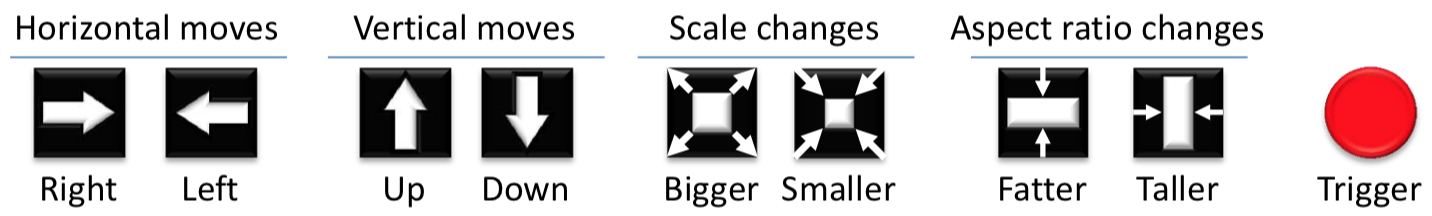
\includegraphics[width=0.7\textwidth]{figures/environment-actions-from-base-paper.png}
    \caption{The actions offered by the environment to the agent\cite{caicedo2015active}}
    \label{fig:environment-actions-from-base-paper}
\end{figure}

The reward function at each step considers the variation of the intersection over the union metric (IoU) and rewards the agent with a discrete $\pm 1$ depending on whether it has improved or not. For the \textit{trigger} action the reward is $\pm 3$ depending on whether the IoU is above a certain threshold. The reasoning behind these rewards is best explained in the paper to which we refer for further explanations and details.

Limits on the duration of episodes and resetting behaviours for the environment are also implemented in the paper in order to avoid situations in which the agent might get lost and lose time for no reason.

